\section{Theory and experimental setup}
\subsection{Metal-semiconductor junctions}
Consider a metal and an $n$-type semiconductor separated from each other, as depicted on the left of \autoref{fig:schottky_barrier}.
\begin{figure}[htbp]
    \centering
    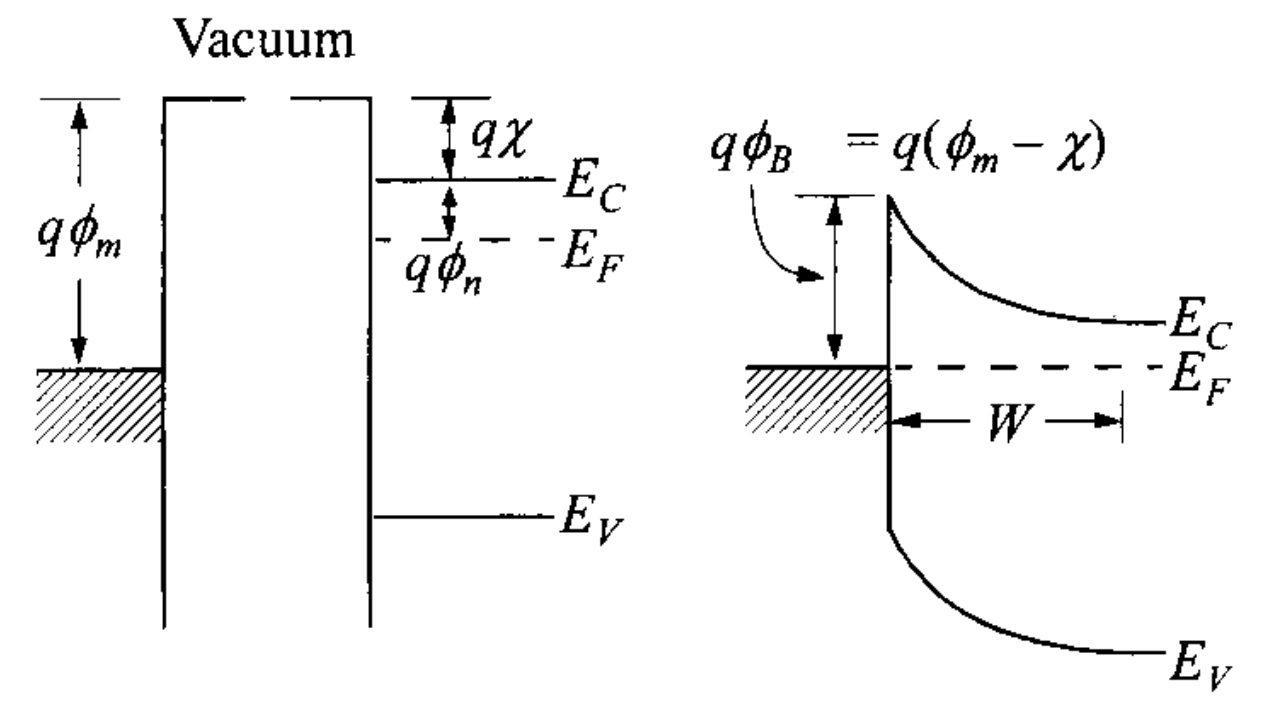
\includegraphics[width=12cm]{figures/schottky_barrier.png}
    \caption{Metal-Semiconductor interface energy levels before (left) and after contact (right) \cite{}}
    \label{fig:schottky_barrier}
\end{figure}
Their work function, defined as the energy difference between the vacuum level and the Fermi level $E_F$, is equal to $q \phi_m$ for the metal, with $q$ the elementary charge, and to $q (\chi + \phi_n)$ for the semiconductor, where $q \chi$ is the electron affinity measured from the bottom of the conduction band energy $E_c$ to the vacuum and $q\phi_n$ is the energy difference between $E_c$ and $E_F$ \cite{sze_physics_2007}.
When the two materials are put in contact, electrons flow from the semiconductor, where the mean energy is greatest, to the metal until their Fermi levels line up.
A negative charge is accumulated in the metal, and a correponding positive one in the semiconductor, causing the formation of an internal electric field and of a potential barrier known as \emph{Schottky barrier} (SB).
For an ideal metal-semiconductor contact, its height \hl{TODO: faudra etre consistant avec ce qu'on appelle la hauteur} $\phi_b$ is the difference between the metal work function and the electron affinity of the semiconductor \cite{sze_physics_2007}:
\begin{equation} \label{eq:barrier_height}
    q\phi_b = q(\phi_m - \chi)
\end{equation}

Though we neglect surface-state effects, \autoref{eq:barrier_height} is generally valid \cite{sze_physics_2007}:
even if the contact is not perfect and a very thin interfacial layer separating metal and semiconductor still remains, this layer is usually so thin ($\sim 10$ \AA) that electrons can easily pass through it by tunnelling \cite{rhoderick_physics_1970}.
More complex models must be applied when the layer is known to be larger.

This barrier gives the junction rectifying properties, as it must be surmounted for the electrons to flow from the metal into the semiconductor.
This behaviour is the basis of an array of electronic components, like Schottky diodes and transistors.

\subsection{Measurement of barrier height}
The Schottky barrier of a Au-Si metal-semiconductor junction was determined using two different methods:

\paragraph{Current-Voltage curves}
The current flow in metal-semiconductor junctions is due to a variety of transport processes.
The principal one is the emission of electrons from the semiconductor over the potential barrier into the metal, as modeled by Bethe's thermionic-emission theory \cite{sze_physics_2007}.
It predicts that the density of current $J$ is tied to voltage $V$ by the equation
\begin{equation} \label{eq:thermionic_emission_current}
    J = J_S \left( e^{\frac{qV}{n k_B T}} - 1 \right), \quad \text{{with}} \quad J_S = A^{**} T^2 e^{-\frac{q \phi_b}{k_B T}},
\end{equation}
where $q$ is the elementary charge, $k_B$ is Boltzmann's constant, $T$ is the temperature of the junction, $n$ is the ideality factor and $A^{**}$ is Richardson's constant.
When conducting measures, one must take into account the sample surface $A$ and the resistance of the junction, modeled by a resistance in series $R$, such that
\begin{equation} \label{eq:iv_curve}
    I = I_S \left( e^{\frac{q (V- RI)}{n k_B T}} - 1\right) = A A^{**} T^2 e^{-\frac{q\phi_b}{k_BT}} \left( e^{\frac{q (V- RI)}{n k_B T}} - 1\right)
\end{equation}

% \begin{equation} \label{eq:IV-curve}
%     V = \frac{n k_N T}{q} \ln \left( \frac{I}{I_S} +1 \right) + RI
% \end{equation}

\hl{APPROVED A bunch of interesting stuff, might add:}
[For electrons ($n$-type Si), $A^{**}$ in the field range $10^4$ to $2\times 10^5$ V/cm remains essentially at a constant value of about 110 \unit{A cm^{-2} K^2}.]

[ A $100 \%$ increase in $A^{**}$ will cause an increase of only $0.018$ V in $\phi_b$. ]


\hl{APPROVED, en plus utile pour modified richardson plot} [Even though $n$ is known as the  "ideality" factor, its numerical value actually reflects the departure from ideality; namely, the larger $n$ is, the less "ideal" is said of the SB \cite{tung_recent_2001}.
Generally speaking, the ideality factor is an indicator of the bias dependence of the SBH \hl{TODO: introduire SBH? remplacer?}. With increasing forward bias, there is a tendency for the effective SBH which controls the current transport to also increase, giving rise to $n > 1$.]


\paragraph{Photoelectric measurement}
Photons carry an energy proportional to their frequency, that is $E = h \nu$.
When an electron absorbs such a photon, it can absorb its energy and reach an excited state.
If this happens in the metal-semiconductor junction, two effects can occur.
If the energy of the photon $h\nu$ is greater than the Schottky barrier energy $\Phi_b := q\phi_b$, the electron can cross the potential barrier, and move with the internal electric field of the junction.
This effect is called internal photoemission.
Therefore, when light at specific frequencies is shone onto the junction, a photocurrent $I$ can be measured across the sample.
This current can be found to be \cite{notice}
\begin{equation}
    I \sim (h \nu - \Phi_b)^2
    \label{eq:fowler}
\end{equation}
If instead the energy of the incident photon excites an electron to an energy larger than the gap between the valence and conduction bands $E_\textrm{gap}$, an effect known as absorbtion occurs.
This creates electron-hole pairs which under the influence of the internal electric field of the junction create a current in the sample.
This phenomenon is the basis of how solar panels work \cite{notice}.

\subsection{Experimental setup}
\paragraph{I-V measures}
The sample, a Au-Si junction of surface area $A = (0.90 \pm 0.07)$ \unit{\cm\squared} was put in a cryostat to lower and control its temperature, which was measured through a Pt100 temperature probe.
To acquire the $I$-$V$ curves, a function generator was set up to sweep the voltage applied on the sample at a frequency of $16$ mHz between $-2.5$ and $2.5$ V while an amperemeter measured the current accross the junction. 
% \hl{For results IMO} Measures were conducted between $124 \pm ?$ and $296\pm?$ K. 

Using least-squares regression, the obtained curves were then fit according to \autoref{eq:iv_curve} to obtain the parameter $I_S$, which is used to derive the barrier height
\begin{equation}
    \Phi_b = k_B T \ln\left(\frac{A A^{**} T^2}{I_s}\right)
\end{equation}
If $\Phi_b$ can be considered independent from the temperature, an alternative derivation using a Richardson plot can be made, by linear regression in a $\ln(I_s/T^2)$ vs $1/T$ plot, derived from \autoref{eq:iv_curve}:
\begin{equation} \label{eq:richardson}
    \ln \left(\frac{I_s}{T^2}\right) = \ln(A A^{**}) - \frac{q \phi_b}{k_B T}
\end{equation}
However, this equation can give wrong results in the case of a non-ideal diode, i.e. for $n \gg 2$. In this case, a modified Richardson plot can be used, for which the equation is modified as \cite{bhuiyan_new_1988}
\begin{equation} \label{eq:modified_richardson}
    n(T) \ln \left(\frac{I_s}{T^2}\right) = \ln(A A^{**}) - \frac{q \phi_b}{k_B T}
\end{equation}

\paragraph{Internal photoemission}
Using a similar setup with a cryostat, light from a monochromator was shone onto the sample, at varying wavelengths.
Due to the monochromator using a diffraction grating to obtain different wavelength, the different filters referenced in \autoref{sec:filters} were used to remove higher order diffractions \hl{BRAZIL? I see your point but it was one of the tasks...}.
A calibration was carried out on each of the filters to correct the measurements on the sample to an equal number of incident photons, by dividing the measured spectra by the calibration spectrum of the selected filter.

After calibration, a plot of $\sqrt{I}$ as a function of the incident photon energy was made, which according to \autoref{eq:fowler} yields a linear relation.
This allows to find the Schottky barrier height $\Phi_b$ at the intercept between the x-axis and a fit of the linear region.
